\chapter{System Implementation} \label{ch:implementation}
\section{Overview of Network Functions} \label{sec:desc_nfv_overview}

While \cite{che-wei-master} focused on the design of vCPE platform, this paper focused on the design of VNF itself.
Our network functions (Fig. \ref{fig:nfv_overview}) are designed with SDN-enabled NFV architecture concept \cite{sdn-enabled}, using the synergies between computer infrastructures (NFVs) and network infrastructures (NFVIs) \cite{etsi-nfv-terminology, etsi-nfv-infra}.
An NFV is mainly used for addressing stateful processing and NFVI is used for stateless processing.
In our architecture, we use an SDN controller as NFV and an SDN switch as NFVI.


\subsection{Stateful Processing Component}
This component is used to control the workflow of network function, maintain the state associated with the VNF, and provide an interface for service providers or customers to configure and update the behavior of the stateless datapath processing component.
We used an SDN controller to implement the VNF controller; and notably, we use southbound APIs of the SDN controller framework to manage the interface between the stateful and stateless components with the OpenFlow protocol, which was originally designed for this purpose.


\subsection{Stateless Processing Component}
Stateless processing component is implemented by SDN datapath resources and is optimized for data plane traffic processing.
Because an SDN switch can be decoupled with control plane and data plane, the switch can accept the control messages from the stateful processing component.

By using the advantages of this architecture, we can assign stateless or light-weight state work to the SDN switch (e.g., packet filtering and packet counting) to reduce the load on the computing resources.
If we want to update our service, we are required to update only the stateful component, because the stateless component merely follows the commands from the stateful component.
\begin{figure}[!t]
\centering
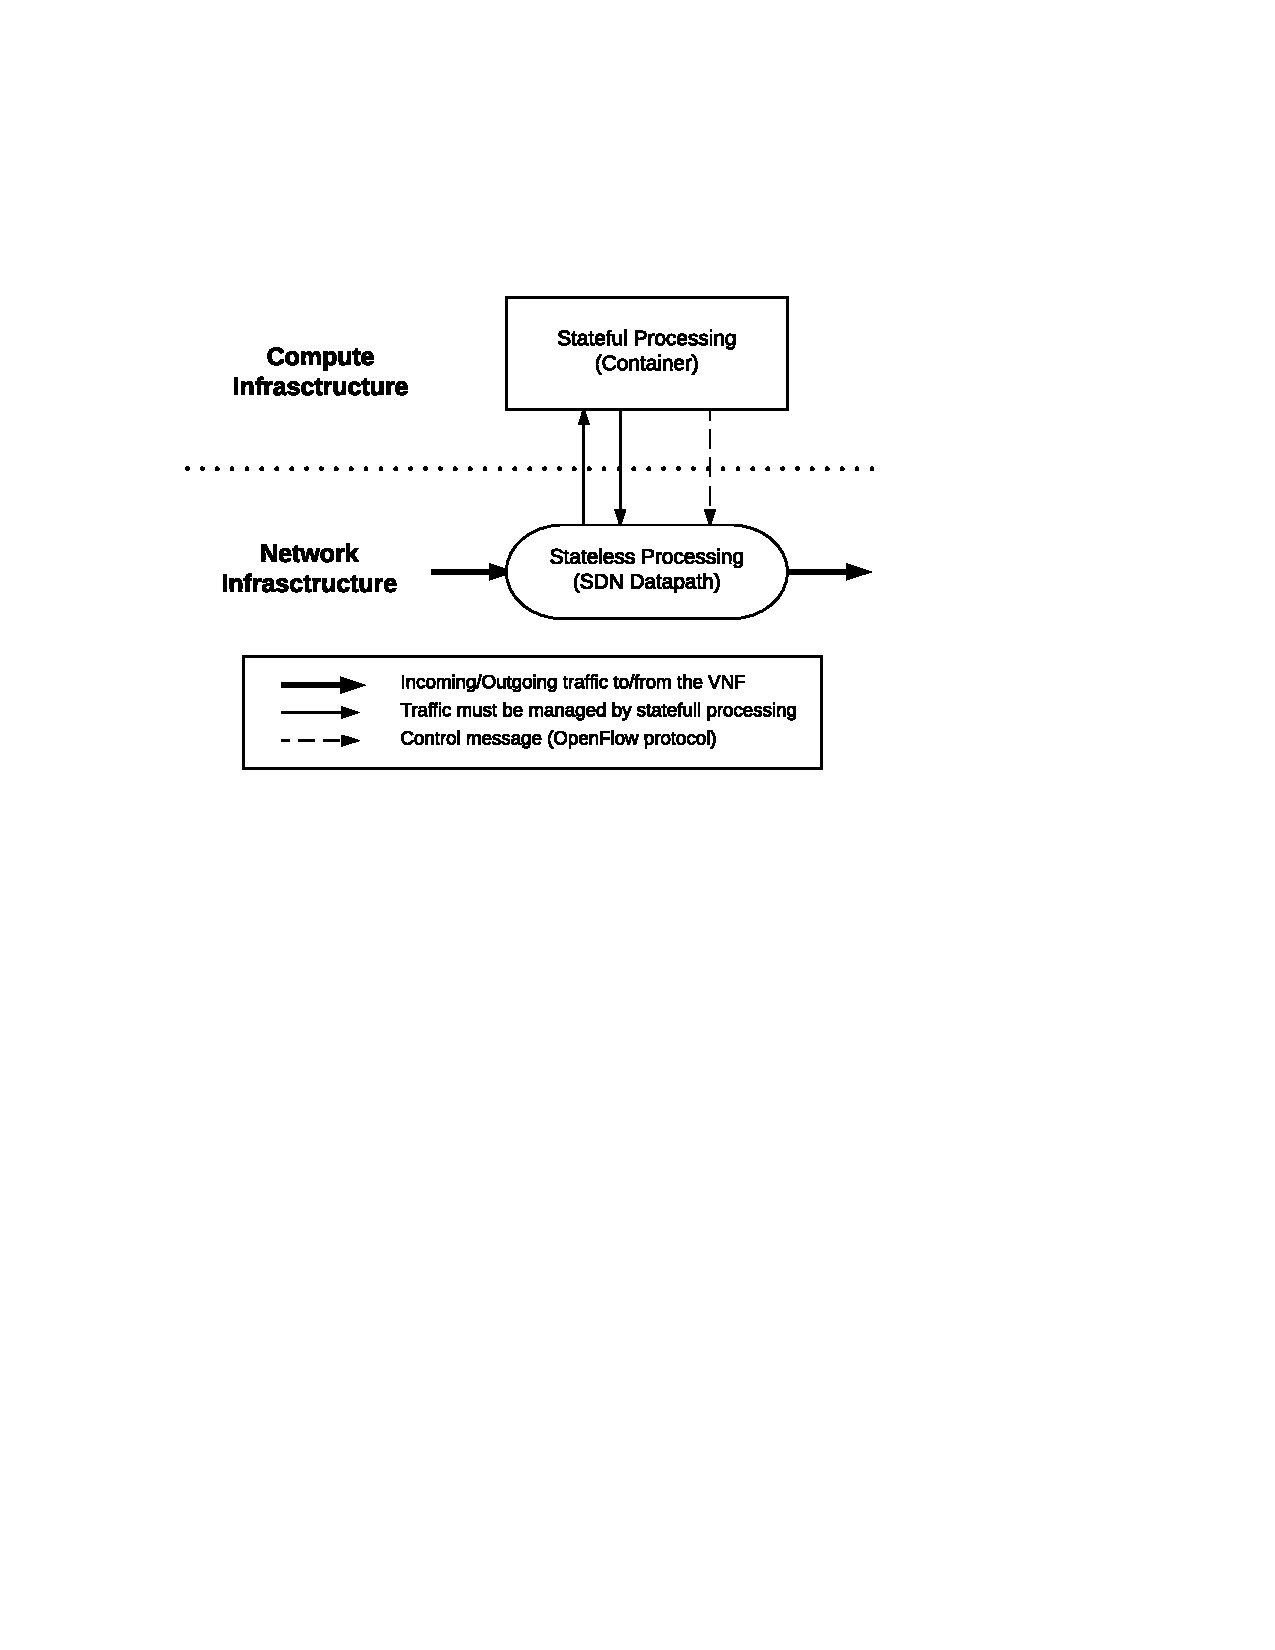
\includegraphics[width=0.7\textwidth]{./fig/nfv_overview}
\caption{Overview of network functions.}
\label{fig:nfv_overview}
\end{figure}


\section{Multiple Flow Table Strategy} \label{sec:multi_flow_table_strategy}

\begin{figure}
\centering
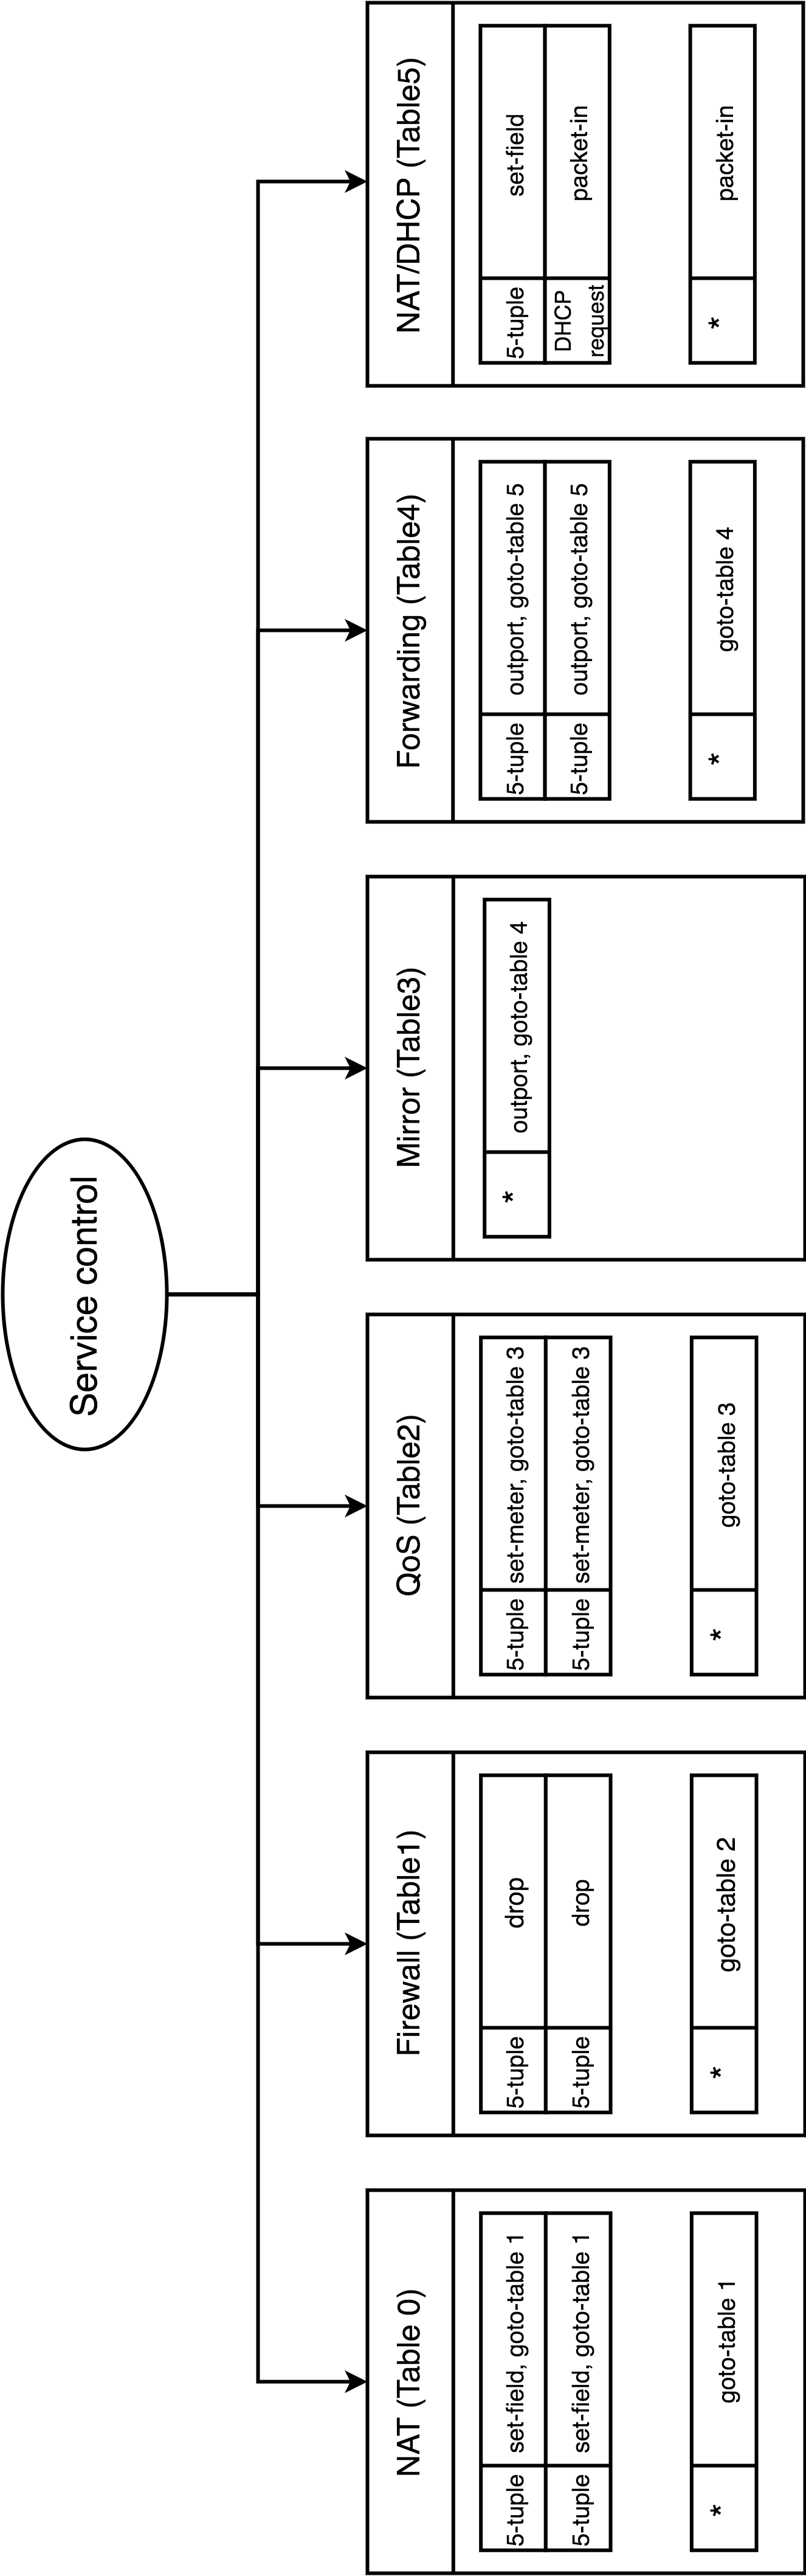
\includegraphics[width=0.4\textwidth]{./fig/mft_table_overview}
\caption{Flow table order of vCPE service.}
\label{fig:mft_table_overview}
\end{figure}

In section \ref{sec:desc_nfv_overview}, we introduce the vCPE service design architecture.
The network functions are achieved by the cooperation between the SDN controller on the cloud and SDN switch at the local network gateway.
The controller transforms the network functions into a series of OpenFlow rule requests and sends them to the SDN switch.
Following the orders from the controller, the SDN switch inserts the rules into its flow tables, examines the incoming packets against the flow entry match fields, and executes the actions in matching rules.
The flow table \cite{sdn-ft} defines all matching and corresponding processing, thus playing an important role in the executive network function.

We found that a single flow table restricts the implementation of our network functions.
In \cite{multiple-flow-table}, two conditions under which a single flow table is too restrictive were reported.
The first is a condition where a single packet must perform independent actions based on matching with different fields.
The second is a condition where the packet requires two-stage processing.
To resolve both restrictions, we implemented the network functions by using a multiple flow table strategy.

The pipeline of OpenFlow flow table was illustrated in Section \ref{sec:openflow}.
In our multiple flow table management mechanism, we set the GOTO-TABLE N action as the table-miss action of table N-1. Therefore, the packet is processed table-by-table in a certain sequence.

In a multiple flow table strategy, it is most important to determine which flow table the rules should be inserted into.
We used the purpose of network function as a demarcation, that is, SDN applications responsible for specific purpose inserted rules into one specific flow table to enable us to focus on the design of the network function itself.
However, the order of the flow table and the sequence of the network functions become crucial.
This can be addressed by considering the type of match and action in the rules generated by the network function.

The network functions of vCPE services are the firewall, NAT, DHCP, forwarding, traffic mirroring and QoS.
The order of each function was determined as shown in Fig. \ref{fig:mft_table_overview} (note that the flow tables are counted from zero).
In the following sections, we introduce the method of implementing these network functions, the type of rules to be inserted into the SDN switch, and the effect of these rules on deciding the order of the flow tables.



\section{Service Control} \label{sec:service_control}

% \begin{figure}[!tp]
%   % \centering
%   \begin{subfigure}[b]{\textwidth}
%     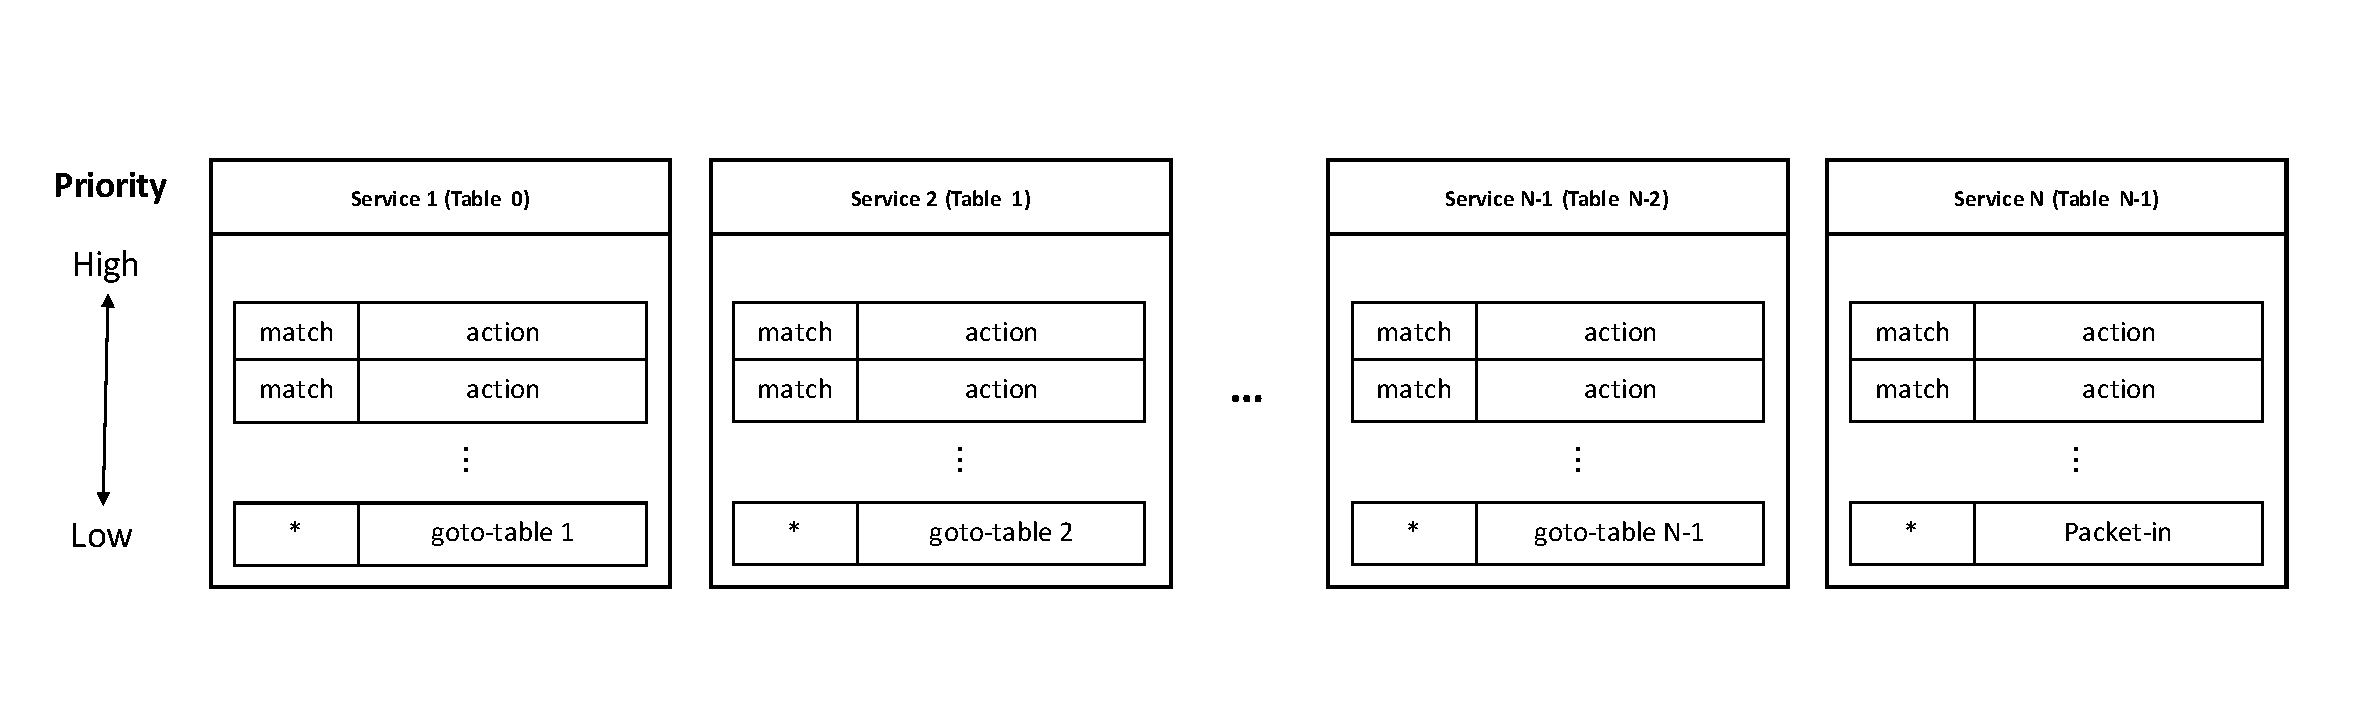
\includegraphics[width=\textwidth]{./fig/service_control1.pdf}
%     \caption{All Services are enabled.}
%     \label{fig:service_control_all_enable}
%   \end{subfigure}
%   \hfill
%   \begin{subfigure}[b]{\textwidth}
%     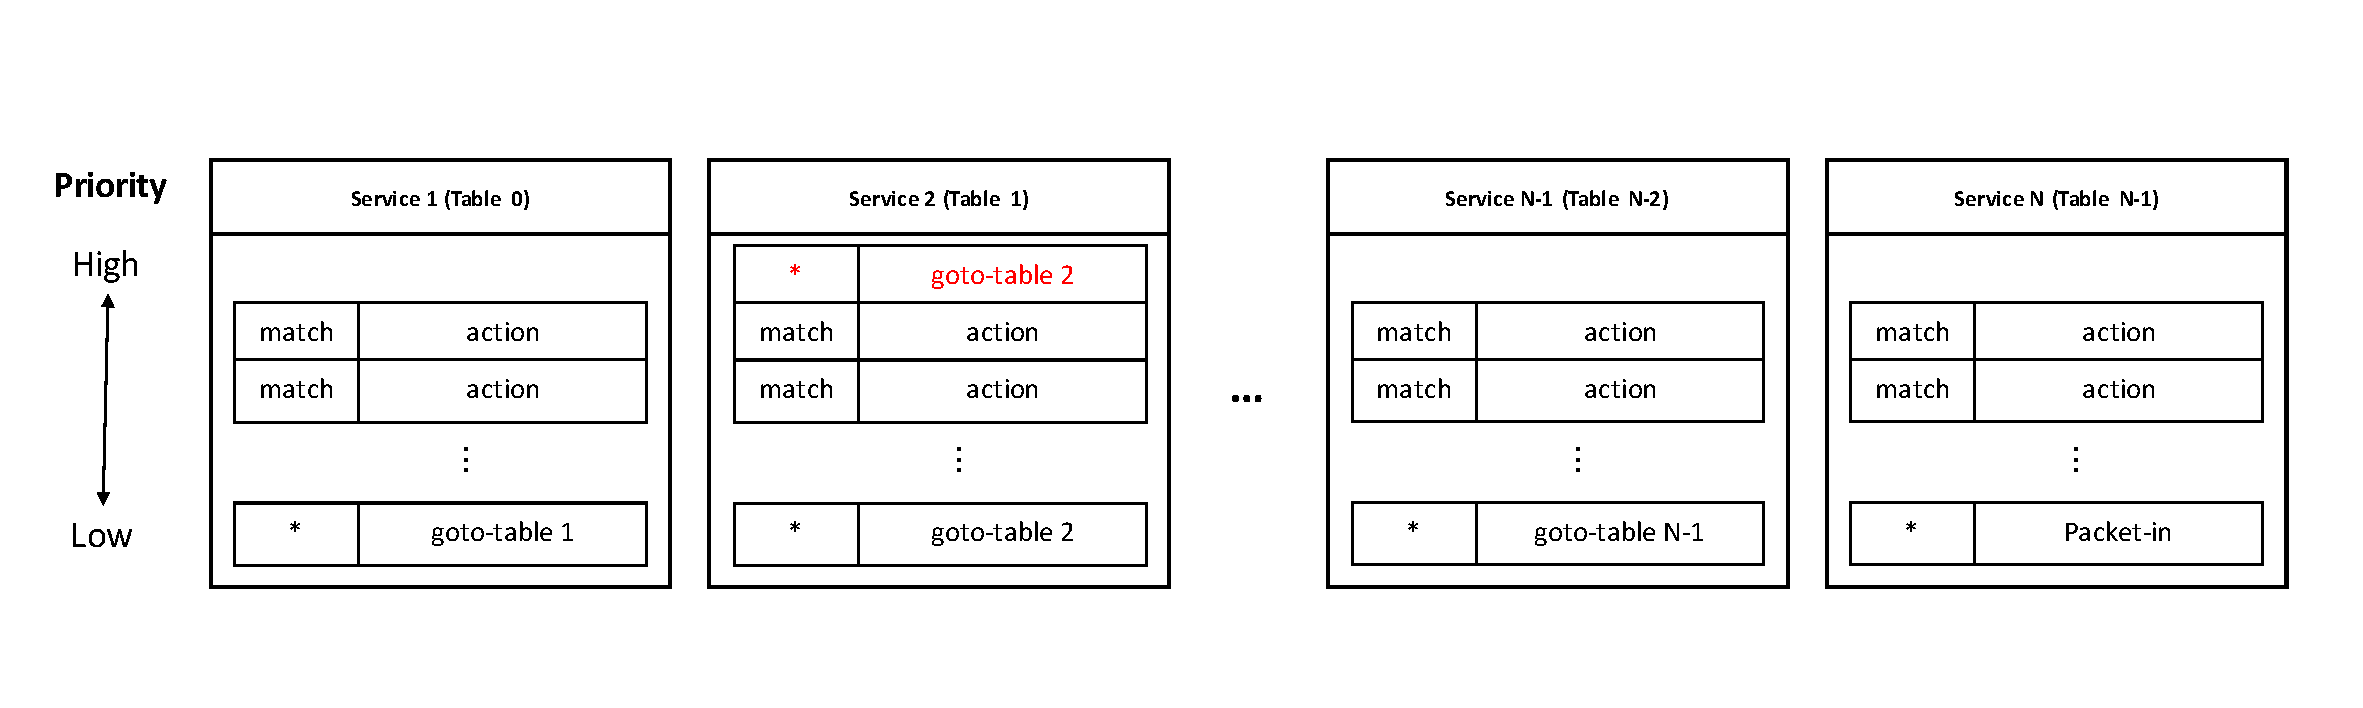
\includegraphics[width=\textwidth]{./fig/service_control2.pdf}
%     \caption{When service 2 is disabled, the force-ignoring rule is added into the table 1.}
%     \label{fig:service_control_disable2}
%   \end{subfigure}
%   \hfill
%   \begin{subfigure}[b]{\textwidth}
%     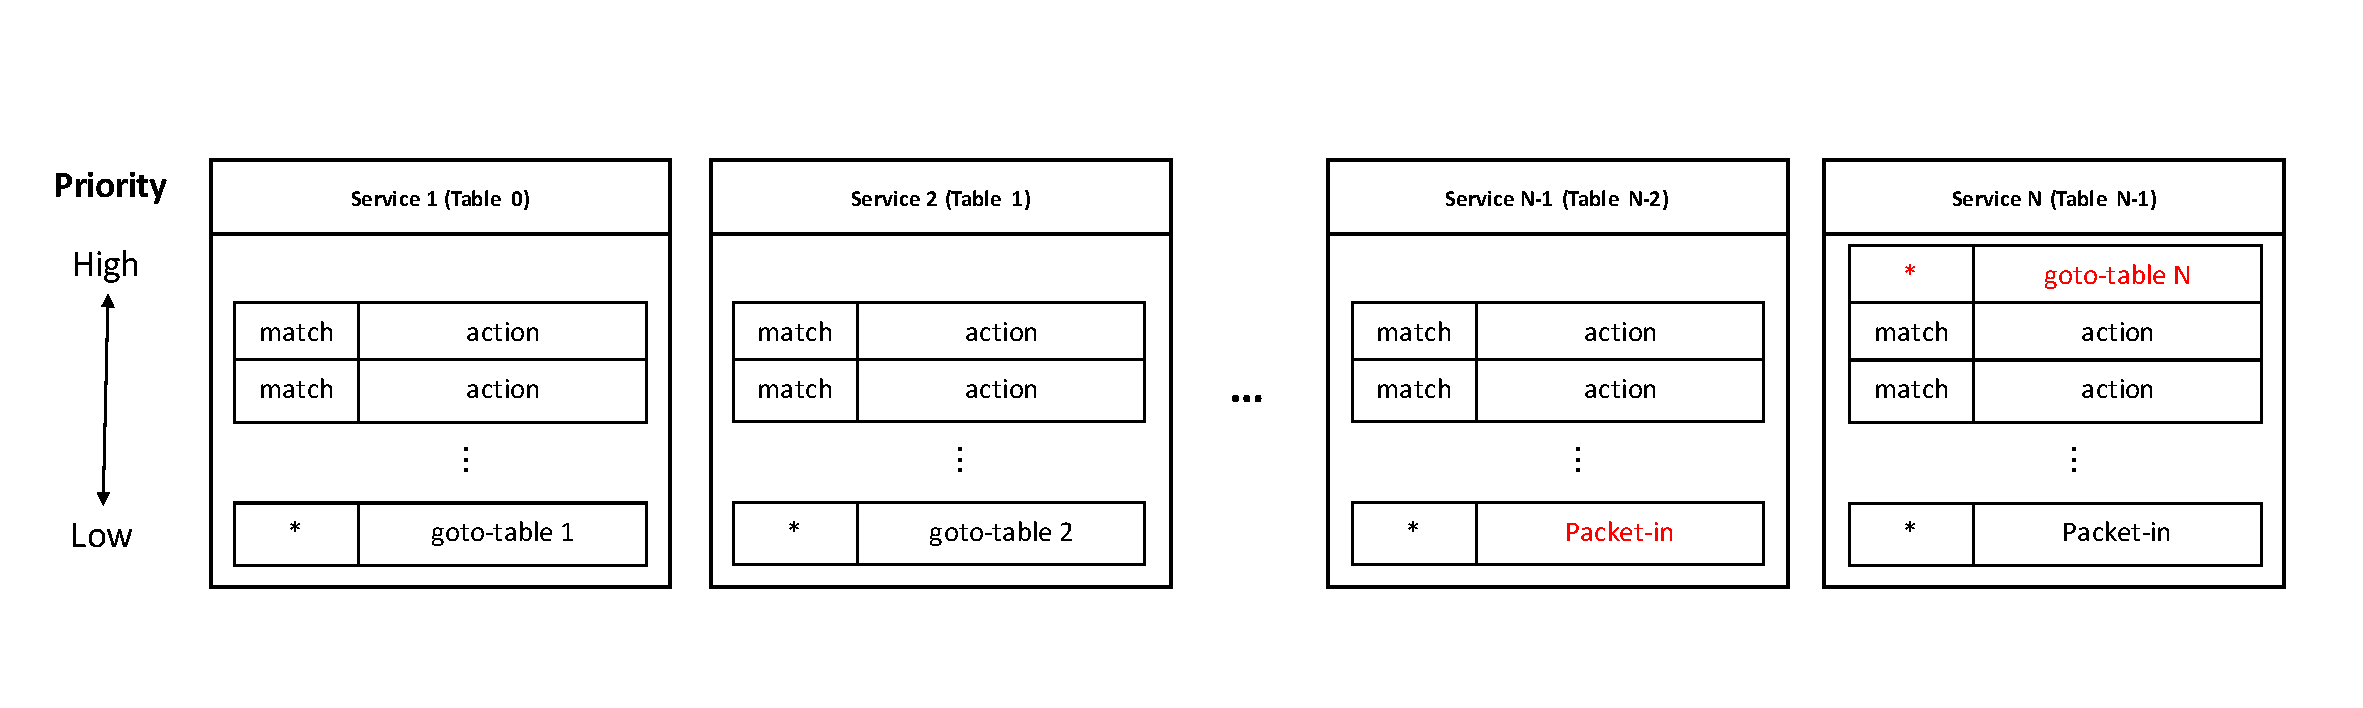
\includegraphics[width=\textwidth]{./fig/service_control3.pdf}
%     \caption{When last service (service N) is disabled, the force-ignoring rule is added into the table N-1 and the PACKET-IN rules is added in to table N-2.}
%     \label{fig:service_control_last}
%   \end{subfigure}
%   \caption{Service control in multiple flow table mechanism.}
% \end{figure}


Service control is used to enable or disable services.
% As shown in Fig. \ref{fig:service_control_all_enable},
A PACKET-IN rule is always placed in the flow table of the last active service as a table miss in case there is no corresponding rule.
To enable the service chain, the rules of each service except the last service contain an additional action GOTO-TABLE, which enables the packets to continue to pass through all active services.

To disable a service, a force-ignoring rule is added into the table of the service.
% (Fig. \ref{fig:service_control_disable2})
The force-ignoring rule has maximum priority with the action GOTO-TABLE.
To enable a service, we just remove the force-ignoring rule.

If the service we want to disabled is located at last table, we must not only modify the force-ignoring rule but also modify PACKET-IN rules.
% The change is shown in Fig. \ref{fig:service_control_last}.


\section{Network functions} \label{sec:setwork_functions}
\subsection{Firewall}
The firewall service can dynamically block traffic and prevent the packets from causing a PACKET-IN event.
On the dashboard, we can specify the blocking policies. There are three kinds of policies:
\begin{enumerate}[leftmargin=4em]
  \item block any traffic from a source IP or destination IP address;
  \item block traffic based on known layer 4 protocols, such as SSH and HTTP;
  \item block traffic with customize layer 4 ports of a host.
\end{enumerate}

For different policies, the controller applies corresponding rules to the SDN switch. After the policies are set, the blocking rules are immediately installed. Subsequently, any traffic that satisfies the blocking criteria is dropped. Normal traffic is unaffected.

As shown in Table \ref{table:fw}, all the actions of flow entries are dropped. The first rule illustrates that SSH connection with the source IP address 192.168.2.1 is blocked. The second rule indicates that the flow entry blocks the Telnet protocol.

In our multiple flow table mechanism, the firewall service is located in flow table 1 because once packets are detected by the blocking rules, they do not need to be applied to any other services. The packets that satisfy the blocking rules are immediately dropped, and their journey in the flow table ends. The other unblocked packets pass all blocking rules and finally satisfy the table-miss rule, which allows the packets to proceed to the next flow table. The action of the firewall is different from those of other services, because in other services, irrespective of the actions taken with the packets, the packets must proceed to the next flow table.

% firewall example table
\begin{table*}[!t]
\caption{Firewall rules in Flow Entry}
\label{table:fw}
\centering
\begin{threeparttable}
\begin{tabular}{|l|l|l|l|l|l|}
\hline
IP proto & IP src      & IP dst       & L4 sport & L4 dport & action \\ \hline
TCP      & 192.168.2.1 & *            & *        & 22       & drop   \\ \hline
TCP      & *           & *            & *        & 23       & drop   \\ \hline
\end{tabular}
  \begin{tablenotes}
    \item[] Symbol * represents wildcard (matches any value).
  \end{tablenotes}
\end{threeparttable}
\end{table*}


\subsection{NAT}
The NAT service allows numerous hosts to use one public IP address for connecting to the network. Following is an example that illustrates the modification of the IP address and port number by using the NAT service. For a new connection, the first outgoing packet can’t match any flow entry in SDN switch, so it will be sent to controller by the PACKET-IN action in the last table. The controller will modify the source IP to the public IP which is set by the network manager and modified the source port to an un-used port. Then, the controller will send the modified packet back to the switch. After that, the controller will send a pair of rule requests to SDN switch: one is for adding rules for egress traffic and the other is for ingress traffic.

There’s an example shown in Fig. \ref{fig:mft_nat}, the public IP address of NAT is 140.114.71.177, and the host private IP address is 192.168.8.254 with the port number 7777. The client sent the packet to a server with the IP address 140.114.71.178 and port number 8080.

As shown in Table \ref{table:nat}, when the host sends the packet to the server (outgoing), a PACKET-IN event is triggered, and the packet is sent to the controller. The set-field action modifies the source IP address to a public IP address of NAT, 140.114.71.177, and the source port to 8888. When the server sends the packet back to the client (incoming), the packet header field is modified. The destination IP address and destination port number are modified to 192.168.8.254 and 7777, respectively.

In the single flow table mechanism, the rules for NAT traffic contains not only SET-FIELD action but also the OUR-PORT action.
We separate the SET-FIELD and OUT-PORT actions into two service: NAT and forwarding.
The benefit of separating two kinds of rules is that the customers can decide enabling or disabling NAT service by themselves.
If they disable the NAT service, they’re still able to connect to the Internet by forwarding service.
The previous NAT service designed by single table mechanism didn’t achieve this flexibility.
In the multiple flow table mechanism, the rules for handling ingress traffic are in the first table and rules for egress traffic are in the last table, since the QoS and forwarding service handle packets with private network packet header when NAT service is enabled.


\begin{figure}[!t]
\centering
\includegraphics[width=0.8\textwidth]{./fig/mft_nat.png}
\caption{Example of modification of IP address and port number by NAT service.}
\label{fig:mft_nat}
\end{figure}

% NAT example table
\begin{table*}[!t]
\caption{Flow entry for modifying the packet header fields}
\label{table:nat}
\centering
\begin{tabular}{|l|l|l|}
\hline
Direction       & Egress          & Ingress         \\ \hline
Table           & 5               & 0               \\ \hline
Match src IP    & 192.168.8.254   & 140.114.71.178  \\ \hline
Match dst IP    & 140.114.71.178  & 140.114.71.177  \\ \hline
Match src port  & 7777            & 8080            \\ \hline
Match dst port  & 8080            & 8888            \\ \hline

Action          & \begin{tabular}[c]{@{}l@{}} src IP $\,\to\,$ 140.114.71.177; \\ src port $\,\to\,$ 8888 \end{tabular}   & \begin{tabular}[c]{@{}l@{}} dst IP $\,\to\,$ 192.168.8.254; \\ dst port $\,\to\,$ 7777 \end{tabular}   \\ \hline
\end{tabular}
\end{table*}



\subsection{DHCP}
The DHCP service implements the DHCP protocol to dynamically assign IP addresses to hosts. A DHCP operation uses the UDP protocol. Clients use port 68 as the source port and port 67 as the destination port. By contrast, the server uses port 67 as the source port and port 68 as the destination port. Our system can handle packets to realize the DHCP service.

This service is executed through the following steps:
\begin{enumerate}
\item The controller adds a DHCP rule for DHCP packets when the service is enabled.
\item All packets match this DHCP rule, causing a PACKET-IN event.
\item If the incoming packet is a DHCP discovery packet, the controller assigns an IP address, generates a DHCP offer, and then performs a PACKEt-OUT event. If the incoming is a DHCP request, the controller generates a DHCP acknowledgement and PACKEt-OUT the generated packet.
\end{enumerate}

Our system supports multiple flow tables; however, a specific flow table for the DHCP service is not required because only one rule is installed for all hosts who request the DHCP service. When the service is disabled, the DHCP rule is deleted, and the packets continue to pass through our service chain. The subsequent DHCP packets can reach other DHCP servers by forwarding service.


\subsection{Forwarding} \label{ssec:forwarding}
In the forwarding service, when the first packet in a new connection is incoming, a PACKET-IN event occurs because no corresponding rule is present. When the controller receives the packet, it records the IP-layer information, including the source IP address, destination IP address, input port number, source MAC address, and destination MAC address. By using the recorded information, the controller can install a 5-tuple forwarding rule with OUT-PORT action for this connection, and the subsequent packets do not need to undergo the PACKET-IN event. The 5-tuple comprises the source IP address, destination IP address, network layer protocol, source layer 4 port, and destination layer 4 port.

The reason why we choose these 5 fields to form 5-tuple is to gather per-session statistical information. The controller installs a pair of dummy rules for every connection, and then requests the switch to obtain current flow statistics every second. Thus, the real-time bandwidth statistics of each connection can be obtained by merely subtracting the byte count from the byte count of the last second.


\subsection{Traffic Mirroring} \label{ssec:mirror}
The traffic mirroring service could make the manager to specify the output port to mirror the packet flow.
It could make the network manager monitor the network situation easily.
In our multiple flow table mechanism, we use this service to mirror the packet flow to classifier which could identify the application.
The QoS service could use the classified result to limit the application.


\subsection{QoS}
QoS is mainly used for traffic control. Two management strategies are provided for QoS. We first introduce two strategies and then discuss the flow table order of QoS in the multiple table model.

\subsubsection{Rate Limitation of Hosts}

To implement the rate limiting for hosts, we use meter table to set the limitation in the specific bandwidth.
With meters, we can create a meter for a desired bandwidth and assign the flows of target host with it.

\subsubsection{Rate Limitation of Applications}
In this strategy, we integrated a flow classification system to identify the flow belongs to which application.  The integration scenario is presented in Fig. \ref{fig:class_classifying}.

To avoid some applications taking up a lot of bandwidth, we can limit the bandwidth for a certain application. We will mirror the packet to flow classification engine and identify which application belongs to. If we want to limit a specific application, we just add a 5-tuple rule and same meter to those packets which belong to this application. As a result, those applications will share the bandwidth by this meter.


\begin{figure}[!t]
\centering
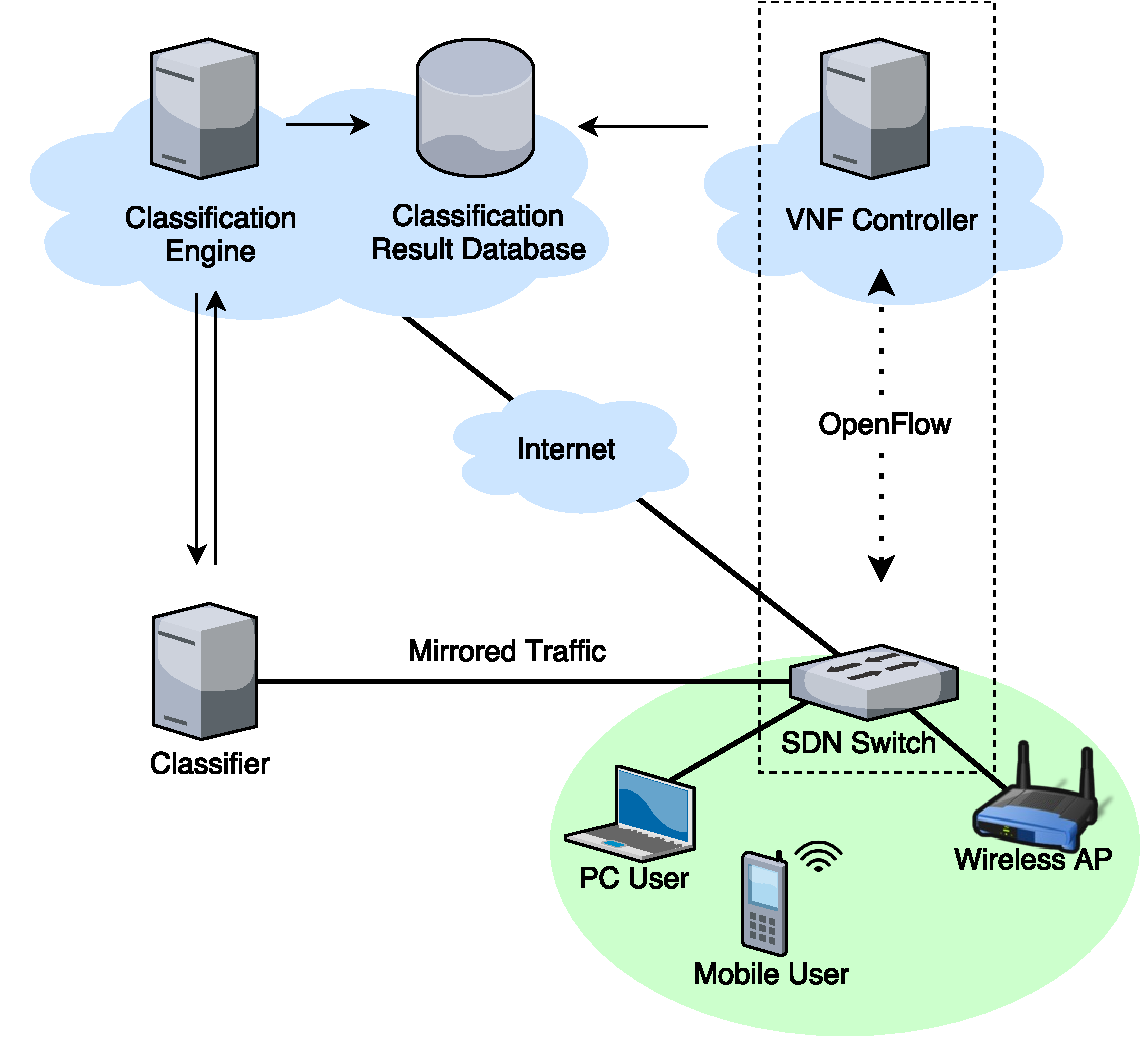
\includegraphics[width=0.9\textwidth]{./fig/classification_classifying}
\caption{Scenario of integration our vCPE function with flow classification system.}
\label{fig:class_classifying}
\end{figure}

\subsubsection{The Flow Table Order of Forwarding and QoS Service}
Because the location of NAT, DHCP, firewall and mirroring have been determined, we only need to decide the arrangement of QoS and forwarding. Assume that we place the QoS flow table after the forwarding flow table. In addition, we have only two services enabled, forwarding and QoS; therefore, the PACKET-IN rule is in the last flow table of active service, QoS service. Then, suppose that a host is not limited by QoS policies. The first packet is not affected in both arrangements. For the subsequent packets, a difference can be observed. The packets that satisfy the rules in the forwarding flow table can not match rate limit rules in QoS flow table, because the host is not limited by QoS service; instead. As a result, the packets cause PACKET-IN events by matching the PACKET-IN rule in QoS service. This is unexpected because the packets already get the out-port action from the forwarding service. That is, it is not necessary to send these packet go to controller, and any PACKET-IN event increases the controller’s load.

To reduce this load on the controller, we place the QoS flow table ahead of the forwarding flow table. In this scenario, all packets that pass through the QoS flow table continue to proceed to the forwarding flow table without satisfying any QoS rules. Then, all packets except the first packet are merely forwarded by the forwarding service instead of causing PACKET-IN events. Thus, the controller’s load decreases.
